\documentclass[10pt,a4paper]{article}
\usepackage[utf8]{inputenc}
\usepackage{amsmath}
\usepackage{gensymb}
\usepackage{amsfonts}
\usepackage{siunitx}
\usepackage[european]{circuitikz}
\usepackage{geometry}
\newgeometry{tmargin=2cm, bmargin=2cm, lmargin=2cm, rmargin=2cm}
\usepackage{amssymb}
\usepackage{multirow}
\usepackage{polski}
\usepackage{graphicx}
\author{\textbf{T. Fąs}}
\title{\textbf{BADANIE FILTRU RLC}}
\begin{document}
\maketitle

\begin{center}
\textbf{\subsection*{STRESZCZENIE}}
\end{center}
Celem doświadczenia było skonstruowanie filtru RLC, zbadanie charakterystyki amplitudowej i fazowej oraz znalezienie częstości rezonansowej dla szeregowego i równoległego połączenia kondensatorów lub cewek. Otrzymane wyniki są zgodne z przewidywaniami.


\begin{center}
\textbf{\subsection*{WSTĘP}}
\end{center}

Filtry RLC składają się z opornika o oporze $R$, kondensatora o pojemności $C$ oraz cewki o indukcyjności $L$. Schemat takiego filtra przedstawiono na Rysunku 1.

\begin{figure}[h!]
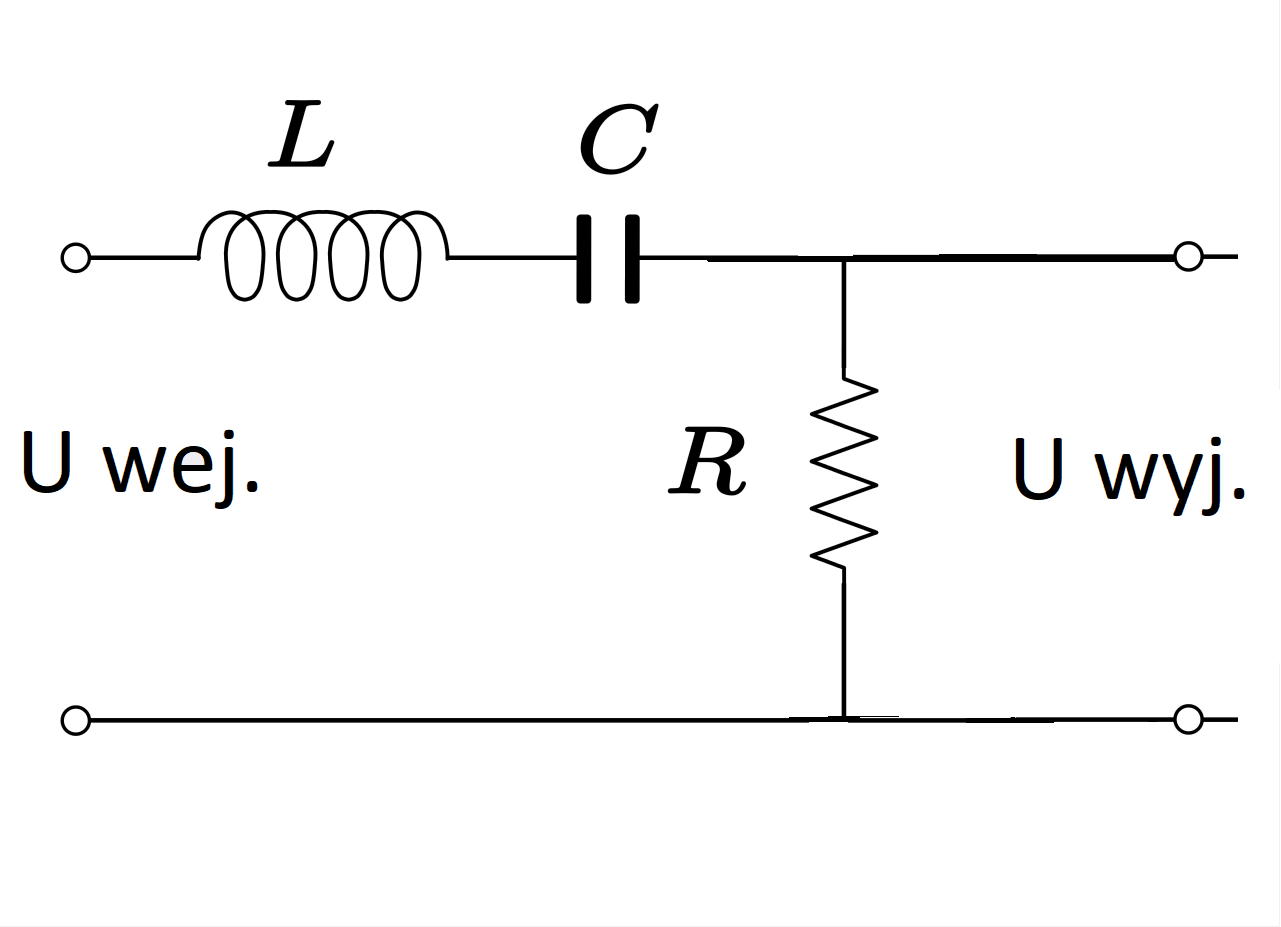
\includegraphics[width=8cm]{rap19rys1} 
\centering
\caption{Schemat obwodu RLC.}
\end{figure}

 Stosunek $T$ amplitudy napięcia wyjściowego $U_{wyj}$ do amplitudy napięcia wejściowego $U_{wej}$ dla obwodu RLC, wraz z uwzględnieniem oporu pasożytniczego $R_{p}$ pochodzącego od cewki i kondensatora, dany jest wzorem:
 
 \begin{equation}
 T=\dfrac{U_{wyj}}{U_{wej}}=\dfrac{R}{\sqrt{\left(R+R_{p}\right)^2+\left(L \omega-\dfrac{1}{\omega C}\right)^2}},
 \end{equation}
 gdzie $\omega$ jest częstością prądu wejściowego.
 
 Z kolei przesunięcie fazowe $\phi$ sygnału wyjściowego względem wejściowego dane jest wzorem:
 
\begin{equation}
\phi=\arctan{\left(\dfrac{1-\omega^2 LC}{\left(R+R_{p}\right)C \omega}\right)}
\end{equation}

Ważnym pojęciem jest częstość rezonansowa $\omega_{rez}=1/\sqrt{LC}$ dla której to transmitancja $T$ przyjmuje wartość maksymalną wynoszącą $R/(R+R_{p})$.

W doświadczeniu badano wartości $T$ oraz $\phi$ dla różnych częstości $\omega$ napięcia wejściowego. Badano również te same wielkości dla innej wartości oporu. Zmierzono również wartości częstości rezonansowej dla układu z dwoma kondensatorami połączonymi równolegle lub szeregowo, jak i dla dwóch cewek łączonych szeregowo bądź równolegle.

\begin{center}
\textbf{\subsection*{UKŁAD DOŚWIADCZALNY}}
\end{center}

Układ doświadczalny składał się z obwodu RLC, złożonego według schematu z Rysunku 1, oscyloskopu oraz generatora sygnałów. Generator został podłączony do obwodu RLC, a dalej do oscyloskopu. Dodatkowo bezpośrednio podłączono generator i oscyloskop, aby móc jednocześnie obserwować sygnał wejściowy i wyjściowy. Schemat układu przedstawiono na Rysunku 2.


\begin{figure}[h!]
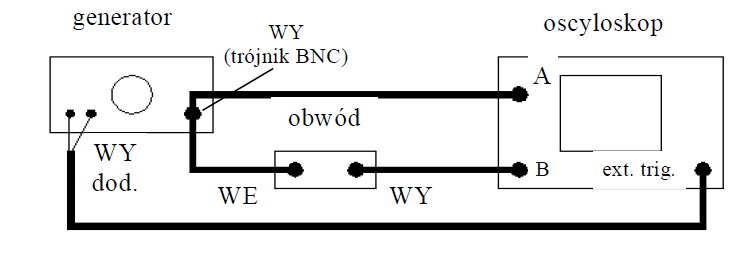
\includegraphics[width=10cm]{rap18rys112} 
\centering
\caption{Schemat układu \cite{r1}.}
\end{figure}

Po zakończeniu pomiarów zamieniono pierwszy opornik na inny, o niżej rezystancji i wykonano ponownie takie same pomiary. Po zakończeniu tej serii, do kondensatora podłączono raz równolegle, a raz szeregowo identyczny kondensator i dla każdego z tych układów zmierzono częstość rezonansową. Podobnie postąpiono w przypadku cewki.

Wszystkie badane wartości były mierzone przy pomocy oscyloskopu, za wyjątkiem częstości prądu, która była odczytywano z generatora.

\begin{center}
\textbf{\subsection*{WYNIKI POMIARÓW}}
\end{center}
Wartości amplitudy napięcia wejściowego, wyjściowego, fazy i częstości są przedstawione w Tabeli 1.

\begin{table}[h!]
\centering
\caption{Wyniki pomiarów.}
\begin{tabular}{|c|c|c|c|c|c|c|c|}
\hline
\multicolumn{4}{|c|}{$R=500,12$ $\Omega$}                           & \multicolumn{4}{c|}{$R=51,6$ $\Omega$}                               \\ \hline
$U_{wej}$ [V] & $U_{wyj}$ [V] & $\phi$ [deg] & $f=\omega/2\pi$ [Hz] & $U_{wej}$ [V] & $U_{wyj}$ [mV] & $\phi$ [deg] & $f=\omega/2\pi$ [Hz] \\ \hline
5,12          & 0,00412       & -180         & 100                  & 5,2           & 0,00284        & -180         & 100                  \\ \hline
5,12          & 0,00608       & -176         & 200                  & 5,16          & 0,00316        & -179         & 200                  \\ \hline
5,12          & 0,0102        & -118         & 500                  & 5,2           & 0,00348        & -179         & 500                  \\ \hline
5,12          & 0,0172        & -96          & 1000                 & 5,2           & 0,00476        & -179         & 1000                 \\ \hline
5,12          & 0,0322        & -91          & 2000                 & 5,2           & 0,0057         & -108         & 2000                 \\ \hline
5,12          & 0,0751        & -88          & 5000                 & 5,16          & 0,0102         & -95          & 5000                 \\ \hline
5,12          & 0,148         & -87          & 10000                & 5,16          & 0,0179         & -91          & 10000                \\ \hline
5,08          & 0,295         & -86          & 20000                & 5,16          & 0,0327         & -90          & 20000                \\ \hline
5,08          & 0,863         & -80          & 50000                & 5,12          & 0,0922         & -89          & 50000                \\ \hline
4,76          & 3,4           & -37          & 100000               & 4,88          & 0,606          & -76          & 100000               \\ \hline
5             & 1,3           & 74           & 200000               & 5,04          & 0,14           & 87           & 200000               \\ \hline
4,88          & 2,6           & -53          & 90000                & 5,04          & 0,344          & -82          & 90000                \\ \hline
4,8           & 3,01          & -46          & 95000                & 5             & 0,441          & -80          & 95000                \\ \hline
4,72          & 3,84          & -25          & 105000               & 4,68          & 0,903          & -67          & 105000               \\ \hline
4,64          & 4,09          & -12          & 110000               & 3,96          & 1,46           & -45          & 110000               \\ \hline
4,64          & 4,09          & 16           & 120000               & 4,48          & 1,14           & 59           & 120000               \\ \hline
4,64          & 4,2           & 3            & 115000               & 3,58          & 1,67           & 22           & 115000               \\ \hline
4,64          & 4,18          & 0            & 113900               & 3,44          & 1,73           & 7            & 113900               \\ \hline
5,04          & 0,34          & 90           & 500000               & 5,04          & 0,0361         & 90           & 500000               \\ \hline
5,04          & 0,0855        & 96           & 1000000              & 5,07          & 0,0106         & 95           & 1000000              \\ \hline
5,08          & 0,174         & 96           & 750000               & 5,04          & 0,0197         & 92           & 750000               \\ \hline
5,08          & 0,259         & 93           & 600000               & 5,04          & 0,0284         & 89           & 600000               \\ \hline
5,04          & 0,463         & 89           & 400000               & 5,07          & 0,049          & 90           & 400000               \\ \hline
4,8           & 3,46          & 38           & 130000               & 4,95          & 0,584          & 75           & 130000               \\ \hline
5             & 1,96          & -63          & 80000                & 5,07          & 0,229          & -86          & 80000                \\ \hline
\end{tabular}
\end{table}

Wartość częstości rezonansowych przedstawione są w Tabeli 2.

\begin{table}[h!]
\centering
\caption{Częstości rezonansowe.}
\begin{tabular}{|c|c|c|}
\hline
             & Równolegle & Szeregowo \\ \hline
Kondensatory & 80,5 kHz   & 160,8 kHz \\ \hline
Cewki        & 160,4 kHz  & 79,8 kHz  \\ \hline
\end{tabular}
\end{table}
 
\begin{center}
\textbf{\subsection*{ANALIZA DANYCH}}
\end{center}

Dla danych z Tabeli 1 obliczono wartości $T$ oraz wykonano wykresy zależności $T(\omega)$ i $\phi(\omega)$. Do tych danych dopasowano zależności kolejno Równania 1 i Równania 2. 
Kierując się instrukcją oscyloskopu za niepewność napięcia przyjęto 2\% z kolei dla pomiarów fazy przyjęto 3$^\circ$ ze względu na wahania tej wartości w trakcie pomiaru.
W trakcie dopasowywania założono, iż $C=0,895$ nF, a $R_{p}=55$ $\Omega$. Wartość $R_{p}$ oszacowano na podstawie wartości częstości rezonansowej z Tabeli 1 ($\phi=0$) i związku $T(\omega_{rez})=R/(R+R_{p})$.

 Dane wraz z krzywymi najlepszego dopasowania przedstawiono na Rysunkach 3-6.



\begin{figure}[h!]
\includegraphics[width=12cm, height=7cm]{rap19rys3} 
\centering
\caption{Dopasowanie: transmitancja $T$ dla $R=500,12$ $\Omega$.}
\end{figure}


\begin{figure}[h!]
\includegraphics[width=12cm, height=7cm]{rap19rys4} 
\centering
\caption{Dopasowanie: faza $\phi$ dla $R=500,12$ $\Omega$.}
\end{figure}

\begin{figure}[h!]
\includegraphics[width=12cm, height=7cm]{rap19rys5} 
\centering
\caption{Dopasowanie: transmitancja $T$ dla $R=51,6$ $\Omega$.}
\end{figure}


\begin{figure}[h!]
\includegraphics[width=12cm, height=7cm]{rap19rys6} 
\centering
\caption{Dopasowanie: faza $\phi$ dla $R=51,6$ $\Omega$.}
\end{figure}

 Wartości parametru $L$ wynikłe z dopasowania przedstawiono w Tabeli 3.

\begin{table}[h!]
\centering
\caption{Wartości indukcyjności.}
\begin{tabular}{|c|c|c|}
\hline
$R$ [$\Omega$]  & 500,12            & 51,6               \\ \hline
Z transmitancji [mH] & $2,25\pm 0,11$  & $2,198\pm 0,061$ \\ \hline
Z fazy     [mH]     & $2,18\pm 0,16$ & $2,198\pm 0,068$  \\ \hline
\end{tabular}
\end{table}

Krzywe sprawiają wrażenie dobrze dopasowanych do punktów i można uznać je za zgodne z teorią. Korzystając z wyznaczonych wartości indukcyjności oraz ze znanej pojemności kondensatora obliczono wartości częstości rezonansowych wraz z niepewnościami. Niepewność pojemności obliczono, korzystając z instrukcji do miernika \cite{m1}. Wartości obliczonych częstości znajdują się w Tabeli 4.

\begin{table}[h!]
\centering
\caption{Częstości rezonansowe.}
\begin{tabular}{|c|c|c|}
\hline
$R$ [$\Omega$]       & 500,12           & 51,6             \\ \hline
Z transmitancji [Hz] & $705401\pm51637$ & $712937\pm42194$ \\ \hline
Z fazy [Hz]          & $715796\pm63742$ & $713044\pm43405$ \\ \hline
\end{tabular}
\end{table}

Założywszy, iż zmierzona wartość częstości rezonansowej wynosi $\omega/(2\pi)=113,9\pm0,2$ kHz, to wszystkie częstości z Tabeli 4 są z nią zgodne na mocy testu 3$\sigma$. Tak więc wyznaczone wartości są zgodne z oczekiwaniami.

Zmierzone częstości rezonansowe z Tabeli 2 również są zgodne z przewidywaniami. Dla połączenia równoległego kondensatorów otrzymana wartość powinna być mniejsza od wartości podstawowej o czynnik $\sqrt{2}$, z kolei dla łączenia szeregowego powinna być większa o ten czynnik. W przypadku cewek sytuacja jest odwrotna: dla łączenia szeregowego częstość jest mniejsza, a dla równoległego większa o $\sqrt{2}$.  

W Tabeli 5 przedstawiono odpowiednio przemnożone wartości. Przy założeniu, że pomiar tych wielkości był obarczony błędem 0,2 kHz, to wszystkie te wartości są zgodne z wartością 113,9 kHz na mocy testu 3$\sigma$.


\begin{table}[h!]
\centering
\caption{Wartości częstości po odpowiednim przemnożeniu.}
\begin{tabular}{|c|c|c|}
\hline
             & Równolegle & Szeregowo \\ \hline
Kondensatory & 113,8 kHz  & 113,7 kHz \\ \hline
Cewki        & 112,9 kHz  & 113,4 kHz \\ \hline
\end{tabular}
\end{table}


Dodatkowo obliczono szerokość pasma przenoszenia, czyli różnicę między dwoma częstościami granicznymi, dla których Równanie (2) przyjmuje wartość $\pi/4$. Obliczenia przeprowadzono, korzystając z wartości indukcyjności $L=2,25$ mH. Otrzymane wartości przedstawiono w Tabeli 6. 


\begin{table}[h!]
\centering
\caption{Częstości graniczne.}
\begin{tabular}{|c|c|c|c|}
\hline
                    & $\omega_{1}$ [Hz] & $\omega_{2}$ [Hz] & Różnica [Hz] \\ \hline
$R=500,12$ $\Omega$ & 94306             & 133652            & 39346        \\ \hline
$R=51,6$ $\Omega$   & 108554            & 116109            & 7556         \\ \hline
\end{tabular}
\end{table}

Tak jak oczekiwano, otrzymana wartość szerokości pasma przenoszenia dla opornika $51$ $\Omega$ jest znacznie niższa, niż dla większego opornika. Dodatkowo, średnia obliczona z częstości granicznych w obu przypadkach zwraca przybliżoną wartość zmierzonej częstości rezonansowej. Tak więc również i te wyniki można uznać za zgodne z przewidywaniami.


\begin{center}
\textbf{\subsection*{DYSKUSJA WYNIKÓW I WNIOSKI}}
\end{center} 

Układ RLC zachowywał się zgodnie z przewidywaniami teoretycznymi, jego częstości rezonansowe, zmierzone i obliczone pokrywały się za sobą dla każdego rozpatrywanego przypadku, transmitancja oraz przesunięcia fazowe również nie przeczyły wyznaczonym wzorom. W każdym przypadku osiągnięto pełną zgodność między wynikami, a oczekiwaniami.

\begin{center}
\begin{thebibliography}{9}

 \bibitem{r1}
 Praca zbiorowa,
 \emph{Instrukcja do ćwiczenia "Badanie szeregowego filtru rezonansowego RLC"},
 FUW, Warszawa, 2018, s. 1.
 
 
 \bibitem{m1}
 Praca zbiorowa,
 \emph{User’s Guide: DM3058 Digital Multimeter},
 RIGOL, 2008, s. 130.

 
 \end{thebibliography}

\end{center}


\end{document}